% Supplement, part 4 (input by supplement.tex): deployment considerations.
\section{Deployment considerations}\label{s:deploy}
This section expands the deployment discussion of the main paper. It makes no security claim beyond those of the previous sections. Fig.~\ref{fig:arch} shows the parties and the running example.

\begin{figure}[h]\centering
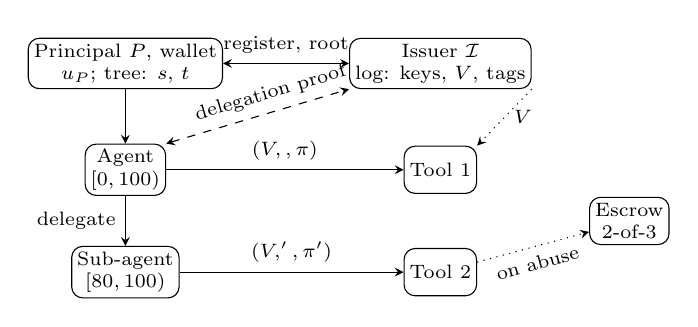
\begin{tikzpicture}[font=\scriptsize,>=stealth,box/.style={draw,rounded corners,align=center,minimum height=6mm,inner sep=2pt}]
\node[box] (P) at (0,2.3) {Principal $P$, wallet\\$u_P$; tree: $s$, $t$};
\node[box] (I) at (4.0,2.3) {Issuer $\mathcal{I}$\\log: keys, $V$, tags};
\node[box] (A) at (0,0.95) {Agent\\$[0,100)$};
\node[box] (S) at (0,-0.35) {Sub-agent\\$[80,100)$};
\node[box] (T1) at (4.0,0.95) {Tool 1};
\node[box] (T2) at (4.0,-0.35) {Tool 2};
\node[box] (E) at (6.4,0.3) {Escrow\\2-of-3};
\draw[<->] (P) -- node[above]{register, root} (I);
\draw[->] (P) -- (A);
\draw[->] (A) -- node[left]{delegate} (S);
\draw[<->,dashed] (A.north east) -- node[sloped,above,pos=0.6]{delegation proof} (I.south west);
\draw[->] (A) -- node[above]{$(V,\nym,\pi)$} (T1);
\draw[->] (S) -- node[above]{$(V,\nym',\pi')$} (T2);
\draw[->,dotted] (I.south east) -- node[right]{$V$} (T1.north east);
\draw[->,dotted] (T2) -- node[below,sloped]{on abuse} (E);
\end{tikzpicture}
\caption{Parties and the running example: the agent holds counters $[0,100)$ per tool and epoch and delegates $[80,100)$ to the hotel sub-agent. The issuer sees root requests and delegations, not presentations.}\label{fig:arch}
\end{figure}


\paragraph{Who runs the issuer, and why tools would accept the cost.} The anonymity set of a presentation is the set of principals of the same issuer whose mandates allow the same call in the same epoch against the same accumulator value. Every tool learns which issuer vouches for the caller. The scheme therefore helps only where one issuer serves many principals whom the tools must not tell apart. Three settings fit:
\begin{itemize}[leftmargin=*]
\item \emph{A platform or federation imposing data minimization on third-party tools.} An agent platform (or a federation of platforms) runs the issuer for all its users and requires tools that only need authorization (search, retrieval, read-only APIs, metered services) to accept presentations instead of user identities, as a contractual condition or to implement data protection by design (GDPR Art.~25). The anonymity set is then the platform's user base for that class and epoch.
\item \emph{A consortium of tools that do not need identity.} Tools that sell per-call access, such as data providers and inference endpoints, can accept the issuer's quota as proof of entitlement and lose nothing by not identifying callers.
\item \emph{A large organization towards external tools.} An enterprise issuer hides which employee or team calls an external tool. Here the tool learns the employer, and the anonymity set is bounded by the number of employees whose mandates allow the class. For a small organization this set may be too small to matter; the scheme then still hides the delegation structure and the call history, but not the organization.
\end{itemize}
Tools that legitimately need the user's identity (payment, delivery, booking under a name) gain nothing from \sys{} for their own calls, and Sec.~VII-D of the main paper shows that they let a coalition name the rest of the session. The running example of the main paper (travel booking with payment) is therefore the case where the scheme helps least: it protects the searches and the sub-agent's activity from tools that do not need the name, and it requires that identity-learning calls be made in a separate session, or at another time, from the rest of the task. E3 measures this: issuing the identity-learning call alone, at a random time within the next hour, cuts naming from 68\,\% to 22\,\% at 1{,}000 users against an attacker that matches amounts only within a short window. An attacker that joins the payment to the earlier quote of the same amount across the whole hour brings naming back to 44\,\% (its join is right 83\,\% of the time); when the decoupled call carries no value echoed from the task, for example a payment against an opaque order token that the search tool never saw, naming stays at 20\,\%. The design rule is therefore that a decoupled call must carry no amount, identifier or date that also appears in the task's other calls or results.

\paragraph{Operational cost for tools.} A tool verifies a presentation of \PresB{}~bytes in about \VerMs{}~ms of one core (the main paper's E1), against well under a millisecond for a JWT. It also keeps two pieces of state that must be shared by all its replicas: the single-use nonces it issued, and the seen-set of pseudonyms for the current epoch. Both are small and short-lived (one entry per call, dropped at the end of the epoch), and fit a shared key-value store with atomic insert (for example \texttt{SET NX} with a time-to-live of one epoch). The reservation of a pseudonym before verification (Sec.~IV of the main paper) makes concurrent verification by several replicas safe as long as the insert is atomic.

\paragraph{Relation to the MCP authorization specification.} Revision 2026-07-28 of the MCP specification requires, when authorization is used over HTTP, an OAuth bearer access token in the \texttt{Authorization} header of every request, issued for the server as audience (RFC~8707), and forbids servers to accept or transit other tokens~\cite{mcpauth}. Our binding carries the presentation in the request's \texttt{\_meta} field and is therefore \emph{outside} the core specification. Two deployment options are compatible with it:
\begin{itemize}[leftmargin=*]
\item \emph{As an authorization extension.} The specification defines optional, additive authorization extensions. A \sys{} extension would let a server advertise that it accepts presentations (with its tool descriptor) and define the \texttt{\_meta} field and the challenge request. Clients that do not implement it fall back to OAuth. In such an extension the nonce request would naturally be a dedicated JSON-RPC method or capability rather than a tool, so that clients unaware of the extension never show it to a model; the specification's extension repository (\texttt{modelcontextprotocol/ext-auth}) is where it would be proposed.
\item \emph{Together with a per-server domain token.} The client presents an ordinary bearer token issued by the domain's authorization server for this server (RFC~8707 audience, no user identity, shared by all principals of the domain), and the presentation in \texttt{\_meta} carries the per-call authorization. The access token then authenticates the domain, not the user; it is a bearer secret shared by many clients, so leaking it exposes only the OAuth layer, not the per-call authorization. If the authorization server issues a token per client instead, that token is a linking handle, and the deployment loses unlinkability towards the tool. We did not evaluate this option.
\end{itemize}
In our MCP binding the nonce request is a separate server operation (a \texttt{challenge} tool) that the client harness calls before each authorized call; it is not listed among the tools offered to the language model, so prompts are unchanged. It costs one extra round trip per call (E2 reports it).

\paragraph{Personal data and the escrow (GDPR).} The following is our reading, not legal advice.
\begin{itemize}[leftmargin=*]
\item \emph{Are presentations personal data for tools?} A presentation is pseudonymous data in the sense of Art.~4(5) GDPR: the escrow committee can attribute it with additional information that the tools do not hold. Under Recital~26 and the Court of Justice's relative approach in \emph{EDPS v SRB} (C-413/23~P, 4~September~2025)~\cite{cjeu2025srb}, and the EDPB's draft guidelines on pseudonymisation~\cite{edpb2025pseudo}, whether such data is personal for a given recipient depends on whether that recipient has means reasonably likely to be used to re-identify the person. A tool without access to the committee's keys may then not be processing personal data through the presentation itself. The call content and timing may still identify the person: E3 shows that a coalition pooling logs re-identifies many calls, so in realistic deployments the tools' logs remain personal data, and the issuer, which knows when delegations happen and which roots it issued, and the committee remain controllers or processors of personal data.
\item \emph{Roles.} The issuer and the platform that operates it determine the purposes and means of authorization and are controllers (jointly, Art.~26, if they decide together). The committee members act for the controller on documented instructions (processors, Art.~28) or as independent controllers if a law gives them their own task. Tools are controllers of the call content they receive.
\item \emph{Lawful basis for an opening.} An opening is a new processing operation and needs its own lawful basis under Art.~6, typically a legal obligation of the controller (Art.~6(1)(c)), which applies only where Union or Member State law compels the disclosure, for example a binding request from a competent authority (whose own processing then falls under Directive (EU) 2016/680), or a legitimate interest in investigating abuse that is not overridden by the principal's interests (Art.~6(1)(f)), assessed case by case.
\item \emph{Notification.} Informing the principal follows from the transparency duties (Arts.~13--14 and 15). It may be delayed or restricted where Union or Member State law allows it under Art.~23, for example during a criminal investigation.
\item \emph{Governance we recommend.} Three committee members independent of the platform and of each other; for every opening request, a log entry before any share is released, holding a commitment to the request and its justification that is opened once any investigation allows it (delayed transparency reconciles public accountability with the confidentiality of criminal investigations under Art.~23 GDPR and Directive (EU) 2016/680); and escrow keys scoped to a period and erased after the retention time, so that old ciphertexts become unopenable. Revocations are part of the scheme: the log accepts them only with an anonymous proof made with the revoked mandate's own credential (held by its holder and its parent) or with two committee signatures. These are design recommendations; the GDPR does not prescribe this committee.
\end{itemize}

\paragraph{Channels outside the cryptographic model.} Names or addresses in call arguments identify the principal (E3 measures how much content reveals). IP addresses and TLS sessions call for a relay such as Oblivious HTTP. The MCP session identifier and client information link the calls of one session; one stateless session per call removes this (E2). An OAuth access token per client identifies it; with \sys{}, tools need no client authentication beyond the presentation, or a token shared by the domain. The issuer sees when roots are issued (identified) and when delegations happen; wallets should reach it through a relay and not request roots right before use, and E3's issuer attacker assumes long-lived roots.

\paragraph{Revocation under a shared issuer (E4).} A presentation built against accumulator value $V$ and verified after a tool installed its successor is rejected when the grace window is zero. Two remedies were measured.
\begin{itemize}[leftmargin=*]
\item \emph{Wallet retry.} After a rejection, if the wallet has seen a newer value, it rebuilds the presentation once against that value, with the same counter and a fresh tool nonce. Reusing the counter is safe for the quota because tools release the reservation of a pseudonym whose proof fails, so a rejected pseudonym is never recorded. It has a privacy cost: the two attempts carry the same pseudonym, so a tool that rejects falsely can link them, and a counter released without a retry must not be reused for a later call to the same tool. Our wallet API enforces this: a released counter is stored with the hash of the call, reused only by the next presentation of the same call to the same tool in the same epoch, and burned otherwise. The unlinkability game does not model retries; for this reason the time-bounded window, not the retry, is the scheme's freshness mechanism (Sec.~IV of the main paper). A first variant that drew a new counter wasted quota (18 of 696 honest calls rejected) and was abandoned. Without either remedy, the scripted agent saw 80 of 460 honest calls rejected (17\,\%), as the LLM agents did, so the effect is not an artefact of the harness.
\item \emph{Time-bounded window.} The tool accepts the previous value only for $\Delta$ after its successor reaches the tool, which bounds the revocation delay by $\Delta$ plus propagation, whatever the revocation rate, and with batching at most two accumulator values coexist at a tool, so the anonymity set splits at most in two; a count-based window $W$ instead delays revocation by $W$ updates, which with sparse revocations means $W$ times their interval.
\end{itemize}
Both remedies avoid honest rejections only while revocations are published less often than a presentation takes to build and reach the tool (about 0.4--0.6~s here); an issuer guarantees this by batching revocations so that it publishes at most one value per $\Delta$. In our runs, new values were pushed to four tools over loopback (about 0.14~s) and the wallet shared the issuer's process, so the delays exclude propagation from the log to real tools and wallets. The scripted runs used a shared, niced login node (Intel Xeon Gold 6426Y), the LLM runs the H100 nodes (Table~\ref{tab:prov}).
